% Options for packages loaded elsewhere
\PassOptionsToPackage{unicode}{hyperref}
\PassOptionsToPackage{hyphens}{url}
%
\documentclass[
  italian,
]{article}
\usepackage{amsmath,amssymb}
\usepackage{lmodern}
\usepackage{iftex}
\usepackage{geometry}
\headsep = -20pt
\textheight = 719pt
\footskip = -10pt
\usepackage{subfig}
\ifPDFTeX
  \usepackage[T1]{fontenc}
  \usepackage[utf8]{inputenc}
  \usepackage{textcomp} % provide euro and other symbols
\else % if luatex or xetex
  \usepackage{unicode-math}
  \defaultfontfeatures{Scale=MatchLowercase}
  \defaultfontfeatures[\rmfamily]{Ligatures=TeX,Scale=1}
\fi
% Use upquote if available, for straight quotes in verbatim environments
\IfFileExists{upquote.sty}{\usepackage{upquote}}{}
\IfFileExists{microtype.sty}{% use microtype if available
  \usepackage[]{microtype}
  \UseMicrotypeSet[protrusion]{basicmath} % disable protrusion for tt fonts
}{}
\makeatletter
\@ifundefined{KOMAClassName}{% if non-KOMA class
  \IfFileExists{parskip.sty}{%
    \usepackage{parskip}
  }{% else
    \setlength{\parindent}{0pt}
    \setlength{\parskip}{6pt plus 2pt minus 1pt}}
}{% if KOMA class
  \KOMAoptions{parskip=half}}
\makeatother
\usepackage{xcolor}
\IfFileExists{xurl.sty}{\usepackage{xurl}}{} % add URL line breaks if available
\IfFileExists{bookmark.sty}{\usepackage{bookmark}}{\usepackage{hyperref}}
\hypersetup{
  pdftitle={Progetto Matlab},
  pdfauthor={Mattia Maglie 1189315; Francesco Marcato 1189319; Marco Martini 1189321},
  pdflang={it-IT},
  hidelinks,
  pdfcreator={LaTeX via pandoc}}
\urlstyle{same} % disable monospaced font for URLs
\usepackage{listings}
\newcommand{\passthrough}[1]{#1}
\lstset{defaultdialect=[5.3]Lua}
\lstset{defaultdialect=[x86masm]Assembler}
\usepackage{graphicx}
\makeatletter
\def\maxwidth{\ifdim\Gin@nat@width>\linewidth\linewidth\else\Gin@nat@width\fi}
\def\maxheight{\ifdim\Gin@nat@height>\textheight\textheight\else\Gin@nat@height\fi}
\makeatother
% Scale images if necessary, so that they will not overflow the page
% margins by default, and it is still possible to overwrite the defaults
% using explicit options in \includegraphics[width, height, ...]{}
\setkeys{Gin}{width=\maxwidth,height=\maxheight,keepaspectratio}
% Set default figure placement to htbp
\makeatletter
\def\fps@figure{htbp}
\makeatother
\setlength{\emergencystretch}{3em} % prevent overfull lines
\providecommand{\tightlist}{%
  \setlength{\itemsep}{0pt}\setlength{\parskip}{0pt}}
\setcounter{secnumdepth}{-\maxdimen} % remove section numbering
\ifXeTeX
  % Load polyglossia as late as possible: uses bidi with RTL langages (e.g. Hebrew, Arabic)
  \usepackage{polyglossia}
  \setmainlanguage[]{italian}
\else
  \usepackage[main=italian]{babel}
% get rid of language-specific shorthands (see #6817):
\let\LanguageShortHands\languageshorthands
\def\languageshorthands#1{}
\fi
\ifLuaTeX
  \usepackage{selnolig}  % disable illegal ligatures
\fi

\title{Progetto Matlab}
\usepackage{etoolbox}
\makeatletter
\providecommand{\subtitle}[1]{% add subtitle to \maketitle
  \apptocmd{\@title}{\par {\large #1 \par}}{}{}
}
\makeatother
\subtitle{Depth Map per ridurre falsi positivi in Face Detection}
\author{Mattia Maglie 1189315 \and Francesco Marcato 1189319 \and Marco
Martini 1189321}
\date{}

\begin{document}
\maketitle

\hypertarget{descrizione-metodo}{%
\section{Descrizione Metodo}\label{descrizione-metodo}}

\hypertarget{descrizione-testuale}{%
\subsection{Descrizione Testuale}\label{descrizione-testuale}}

Data la matrice DepthDATA, considero per ogni elemento il campo (di
indice 2) contenente la matrice di valori di profondità.

Dalla matrice viene poi presa la riga centrale dalla quale vengono tolti i valori a 0 (che indicano un errore del sensore) e su cui vi si effettua
una ``regressione parabolica''. Per la
regressione parabolica si usa la funzione fit del Curve Fitting Toolbox.

Sui coefficienti del curve fit vengono applicate 3 tecniche diverse:

\begin{enumerate}

\item
\textbf{PARABOLIC EXISTENCE}
\newline
Controllo che il risultato del fit sia una parabola. Nel caso in cui non sia una parabola infatti, il calcolo del vertice (-b/2a) restituisce NaN, in quanto il coefficiente di 2° grado è 0 e si ha una divisione per 0.
Se non è una parabola contrassegno direttamente l'elemento come \emph{NonFace}.
Questa tecnica a sé ha una Precision del 100\%.

\item
\textbf{CONCAVITY CHECK}
\newline
Nel caso in cui sia una parabola, controllo che questa sia concava.
Nel caso di parabola concava ho il coefficiente a > 0.
Quindi se il coefficiente a è minore o uguale a 0 contrassegno l'elemento come \emph{NonFace}.
\newline
Precision circa del 94,6\%.

\item
\textbf{VERTEX POSITION}
\newline
Se i primi due controlli vengono superati, avendo quindi una parabola concava, controllo che il vertice di questa sia all'interno di un range specifico:

\(A = matrixHCenter - marginRate \cdot matrixWidth\)

\(B = matrixHCenter + marginRate \cdot matrixWidth\)

Dove \(matrixHCenter\) è la posizione della colonna centrale della
matrice di profondità e \(matrixWidth\) è la larghezza della matrice.

Il coefficiente marginRate arbitrario indica quanto ci si distanzia
dal centro della matrice nel considerare i margini.

Nel caso in cui il vertice della parabola ottenuta con regressione
parabolica si trovi all'esterno del range definito dai due margini allora contrassegno l'immagine come \emph{NonFace}, altrimenti
come \emph{Face}.

La Precision in questo caso varia al variare di \emph{marginRate}
\end{enumerate}

I 3 metodi vengono combinati attraverso l'operatore logico OR.\\
Nel caso almeno uno dei 3 metodi identifichi l'elemento come NonFace, contrassegno il pattern come NonFace altrimenti contrassegno come Face.\\
\\
Combinando i metodi in questo modo, si ha come upperbound della Precision quello del CONCAVITY CHECK, ovvero circa il 94,6\%.

\pagebreak

Si può notare infatti che un'immagine Face ha tendenzialmente valori più bassi
(quindi più vicini alla camera) verso il centro della matrice (causati
dalla presenta della faccia, del naso, ecc.), cosa che non avviene nel caso di una NonFace:

\begin{figure}
\centering
\subfloat[\centering Face]{{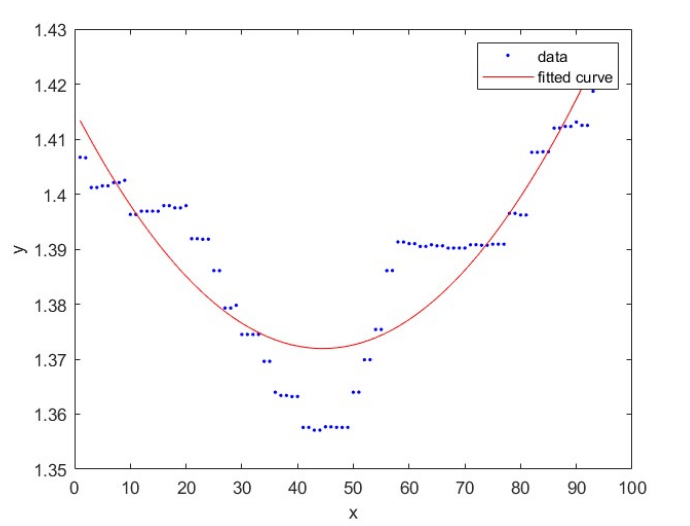
\includegraphics[width=7cm]{img/Face.png} }}%
\qquad
\subfloat[\centering NonFace]{{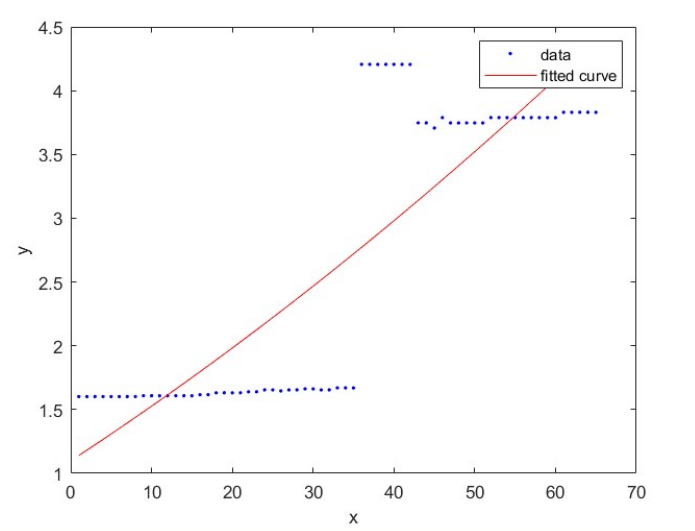
\includegraphics[width=7cm]{img/NonFacce.png} }}%
\caption{Confronto di Face e NonFace}
\end{figure}

Si nota inoltre che la parabola di una Face è per forza di cose convessa.
\newline

Il marginRate è stato invece scelto sulla base del miglior compromesso tra Precision e Recall.

\begin{figure}
\centering
\subfloat[\centering Precision e Recall con marginRate tra 0 e 2]{{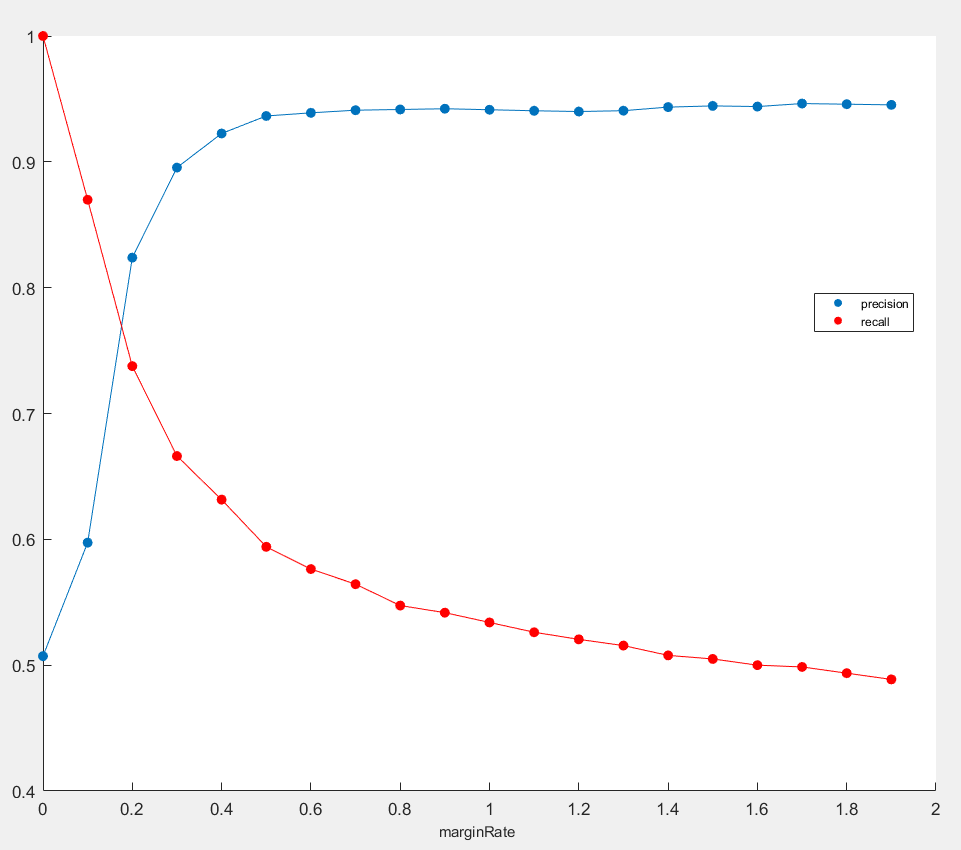
\includegraphics[width=7cm]{img/testingGraph_0_2.png} }}%
\qquad
\subfloat[\centering Precision e Recall con marginRate tra 0.4 e 0.8]{{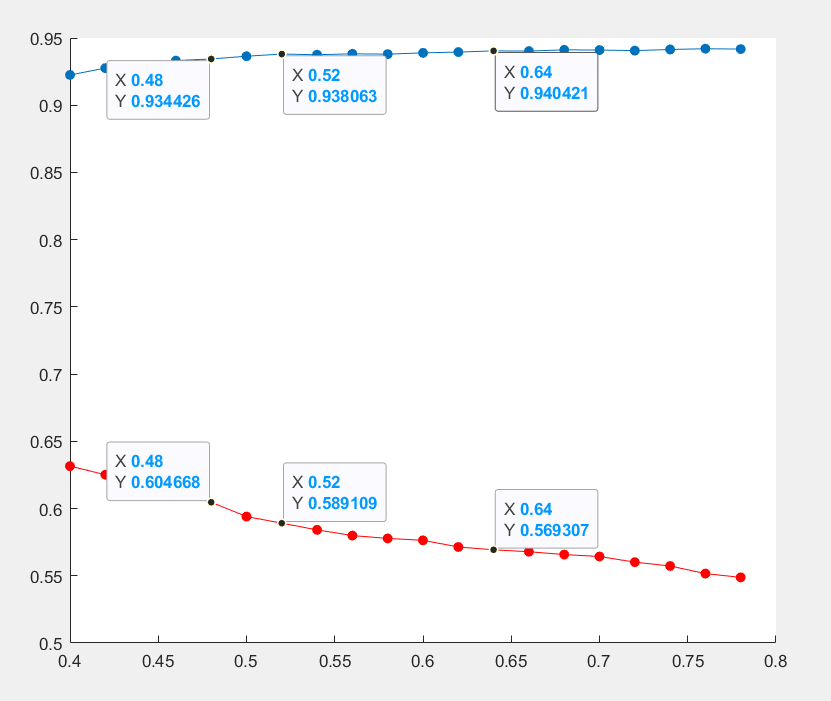
\includegraphics[width=7cm]{img/testingGraph_0_4_0_8.png} }}%
\caption{Scelta marginRate}
\end{figure}

Come si può vedere nel grafico all'aumentare del marginRate la Precision
aumenta a discapito del Recall.

E' stato scelto per questo come compromesso un marginRate di 0,48 che permette un Recall del 60,4\% ed una Precision di 93,4\%.

\pagebreak 

\hypertarget{pseudocodice}{%
\subsection{Pseudocodice}\label{pseudocodice}}

\begin{lstlisting}[basicstyle=\small]
marginRate = 0.48;
Per ogni elemento con indice i di DepthDATA:
  matrix = DepthDATA{i}{2}; 
  matrixVCenter = round(size(matrix, 1)/2);
  centralrow = matrix(matrixVCenter,:);
  x = 1:size(centralrow,2); //creazione indici
  y = transpose(centralrow);
  clearZeros(x, y); //rimozione degli zeri da y e relativo indice x
  f = parabolic_fit(x, y);
  coefficientValues = round(coeffvalues(f), 15);
  vertice = -coefficientValues(2)/(2 * coefficientValues(1)); // -b/2a
  matrixHCenter = round(size(matrix, 2)/2);
  marginA = matrixHCenter - marginRate*size(matrix, 2);
  marginB = matrixHCenter + marginRate*size(matrix, 2);
  
  if(vertice == 0 or vertice < marginA or vertice > marginB or coefficientValues(1) <= 0):
      //contrassegno come NonFace
  else:
      //contrassegno come Face
\end{lstlisting}


\hypertarget{analisi-complessituxe0-temporale}{%
\section{Analisi Complessità
Temporale}\label{analisi-complessituxe0-temporale}}

Per analizzare la complessità del metodo si tiene conto della
complessità temporale delle seguenti funzioni utilizzate:

\begin{itemize}
\tightlist
\item
  size \(= O(1)\)
\item
  transpose \(= O(1)\)
\item
  fit \(= O(1)\)
\item
  clearZeros \(= O(\sqrt[2]{m}) \)
\end{itemize}

Per ognuna delle precedenti funzioni sono stati calcolati i vari tempi
di esecuzione al variare della quantità di dati utilizzati, i risultati
hanno portato alle precedenti conclusioni.

D'ora in avanti considereremo:

\begin{itemize}
\tightlist
\item
  n = numero di immagini
\item
  m = dimensione totale dell'immagine
\end{itemize}

Il metodo quindi ha complessità temporale pari a \(O(n \cdot \sqrt[2]{m})\) in
quanto viene effettuato il fit solo sulla riga centrale e non vengono analizzati tutti gli elementi della matrice.

\hypertarget{risultati-e-prestazione-del-metodo}{%
\section{Risultati e Prestazione del
metodo}\label{risultati-e-prestazione-del-metodo}}

Come detto in precedenza, il metodo ha una Precision e Recall che varia al variare del marginRate.
Con il marginRate scelto, ovvero 0,48 si ottiene:

\(True Positive = 855\) (NonFace individuate)

\(False Positive = 60\) (Face scambiate per NonFace)

\(True Negative = 1314\) (Face individuate)

\(False Negative = 559\) (NonFace scambiate per Face)

\bigskip
Il metodo ottiene quindi i seguenti risultati in termini di recall e
precision:

\(Precision = \frac{TruePositive}{TruePositive + FalsePositive} = \frac{855}{855+60} = 0.9344 \approx 93\%\)

\(Recall = \frac{TruePositive}{TruePositive + FalseNegative} = \frac{855}{855+559} = 0.6046 \approx 60\%\)

\pagebreak

Nel caso si vogliano ridurre al minimo i Falsi Positivi (meno di 10), è possibile farlo combinando solo i metodi 1 (PARABOLIC EXISTENCE) e 2 (VERTEX POSITION).
Facendo infatti così e usando come marginRate 1,69 si ottiene:

\(True Positive = 375\) (NonFace individuate)

\(False Positive = 9\) (Face scambiate per NonFace)

\(True Negative = 1365\) (Face individuate)

\(False Negative = 1039\) (NonFace scambiate per Face)

Ottenendo:

\(Precision = \frac{TruePositive}{TruePositive + FalsePositive} = \frac{375}{375+9} = 0.9765 \approx 98\%\)

\(Recall = \frac{TruePositive}{TruePositive + FalseNegative} = \frac{375}{375+1039} = 0.2652 \approx 27\%\)

Purtroppo in questo caso la Precision alta è a discapito del Recall.

\hypertarget{Analisi degli errori}{%
\subsection{Analisi degli errori}\label{Analisi degli errori}}

Di seguito vengono mostrate due immagini contrassegnate come FalsePositive(Face individuate come NonFace).

\begin{figure}
\centering
\subfloat[\centering immagine a colori senza cornice aggiuntiva]{{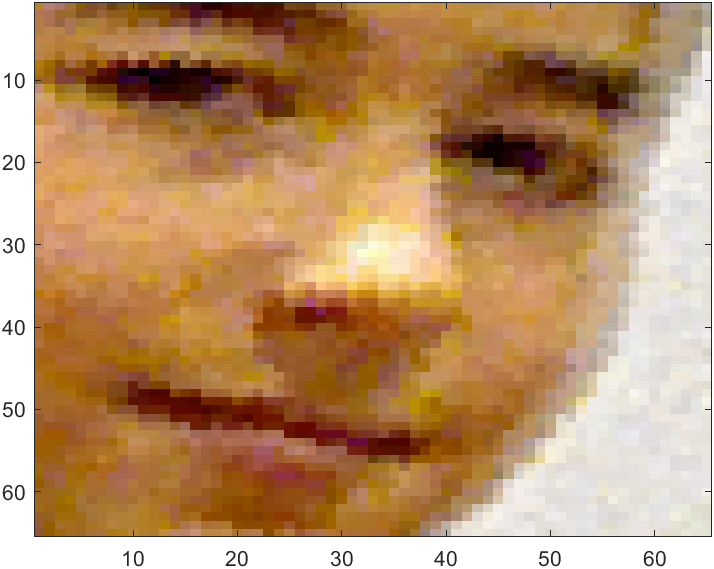
\includegraphics[width=4cm]{img/229-1.png} }}%
\qquad
\subfloat[\centering immagine a colori dell'area relativa alla depth map con "cornice aggiuntiva"]{{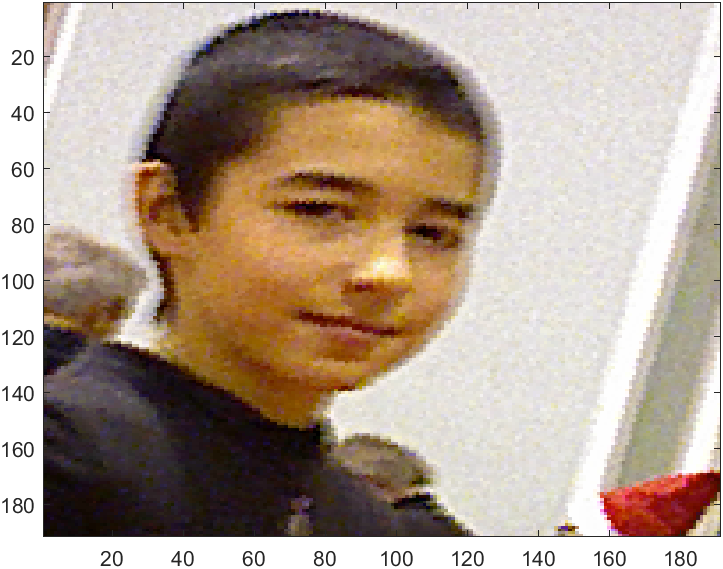
\includegraphics[width=4cm]{img/229-2.png} }}%
\qquad
\subfloat[\centering Regressione parabolica sulla riga centrale una volta tolti i valori a 0]{{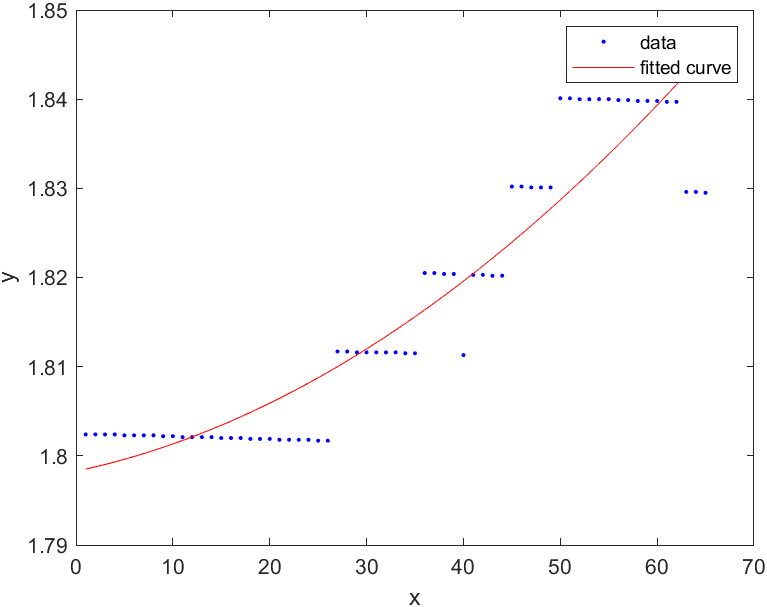
\includegraphics[width=4cm]{img/229-3.png} }}%
\caption{Immagine 229}
\end{figure}
Nella figura 3 si può notare che il metodo non funziona correttamente quanto non è presente tutto il viso nell'immagine senza cornice.
In questo caso infatti il vertice della regressione parabolica si trova a circa -15.

\begin{figure}
\centering
\subfloat[\centering immagine a colori senza cornice aggiuntiva]{{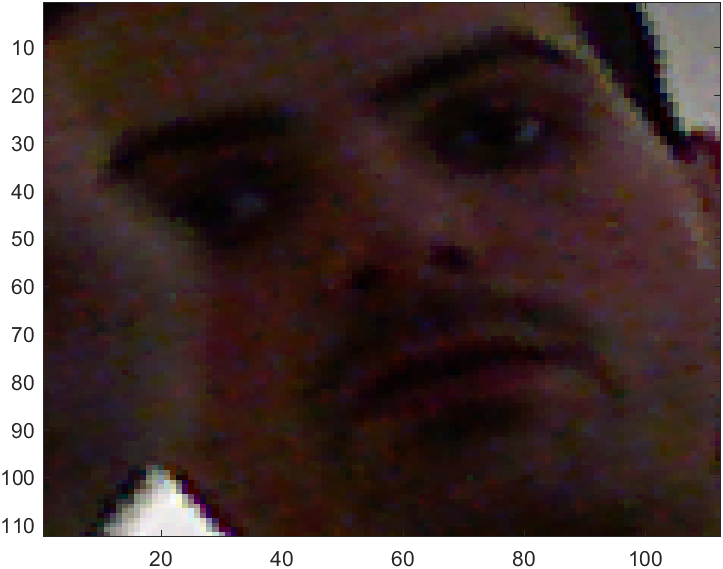
\includegraphics[width=4cm]{img/458-1.png} }}%
\qquad
\subfloat[\centering immagine a colori dell'area relativa alla depth map con "cornice aggiuntiva"]{{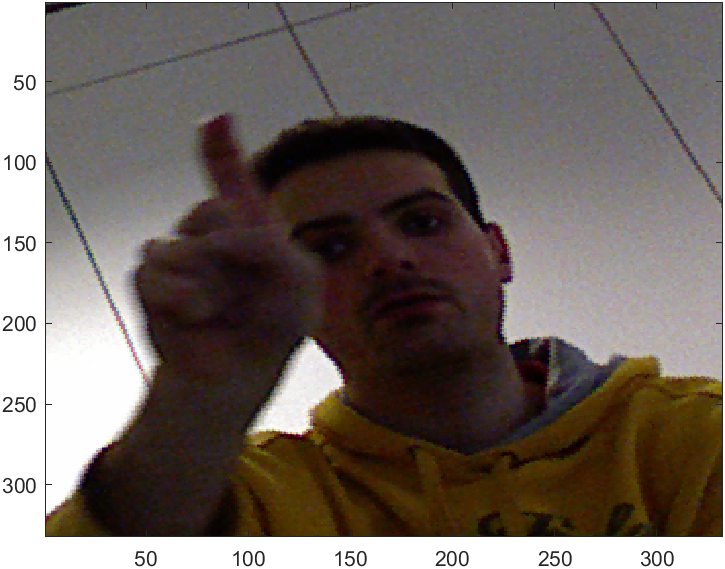
\includegraphics[width=4cm]{img/458-2.png} }}%
\qquad
\subfloat[\centering Regressione parabolica sulla riga centrale una volta tolti i valori a 0]{{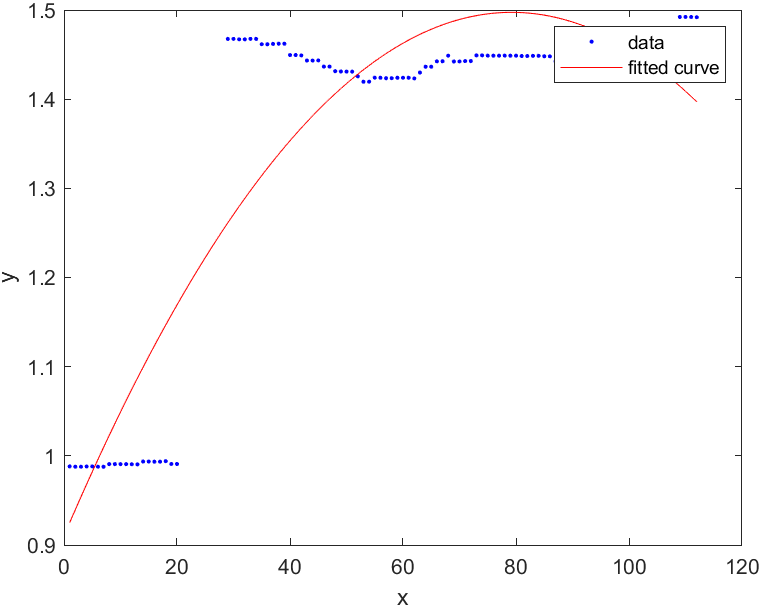
\includegraphics[width=4cm]{img/458-3.png} }}%
\caption{Immagine 458}
\end{figure}
Nella figura 4 si può notare che il metodo non funziona correttamente quanto è presente un oggetto che copre parzialmente il volto.
In questo caso infatti la regressione parabolica non soddisfa il concavity check.

\pagebreak

Ora invece verranno analizzate due immagini contrassegnate come FalseNegative (NonFace individuate come Face).

\begin{figure}
\centering
\subfloat[\centering immagine a colori senza cornice aggiuntiva]{{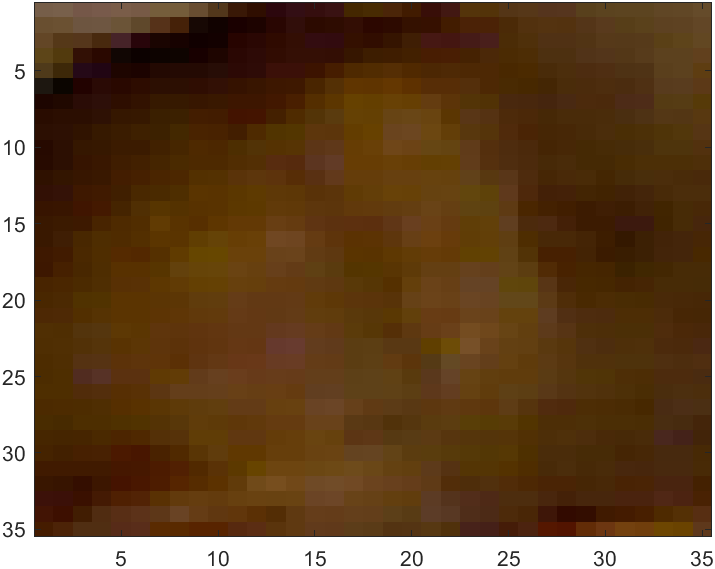
\includegraphics[width=4cm]{img/75-1.png} }}%
\qquad
\subfloat[\centering immagine a colori dell'area relativa alla depth map con "cornice aggiuntiva"]{{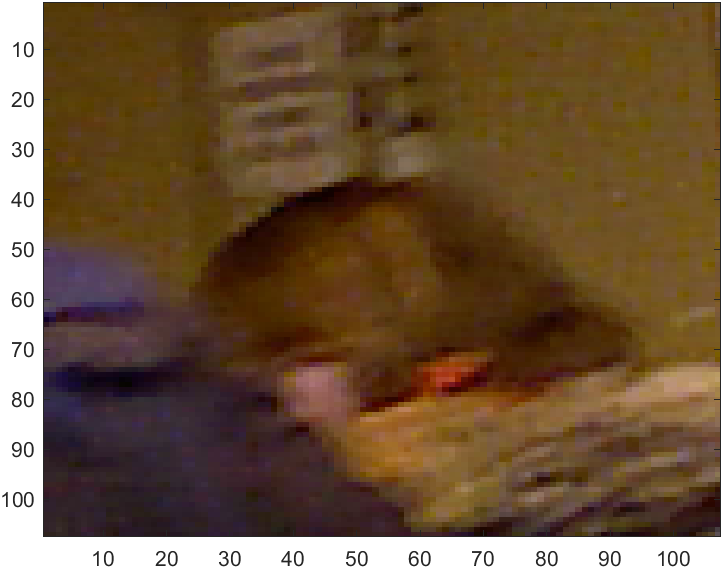
\includegraphics[width=4cm]{img/75-2.png} }}%
\qquad
\subfloat[\centering Regressione parabolica sulla riga centrale una volta tolti i valori a 0]{{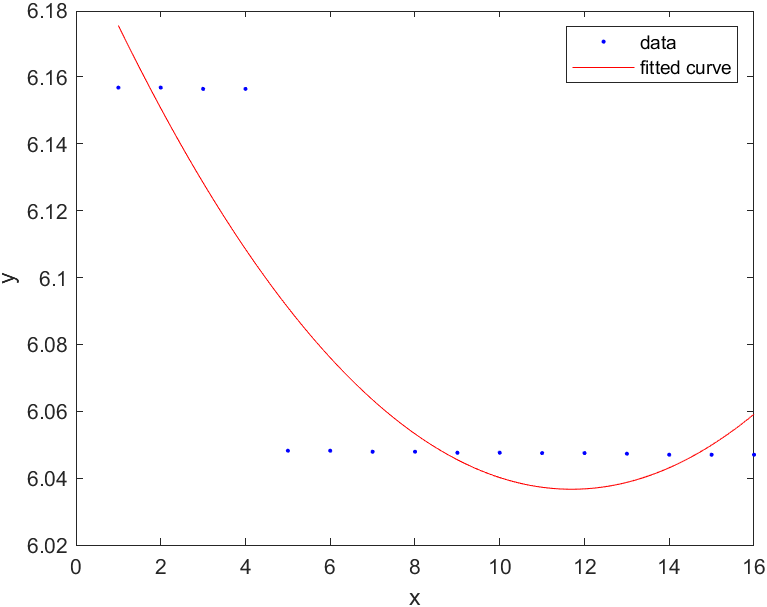
\includegraphics[width=4cm]{img/75-3.png} }}%
\caption{Immagine 75}
\end{figure}
La figura 5 mostra un caso in cui un oggetto di dimensione medio/piccola è posizionato al centro dell'immagine, questo infatti fa in modo che il metodo lo riconosca come Face perchè la sua regressione parabolica è pressochè indistenguibile da quella di una vera Face.

\begin{figure}
\centering
\subfloat[\centering immagine a colori senza cornice aggiuntiva]{{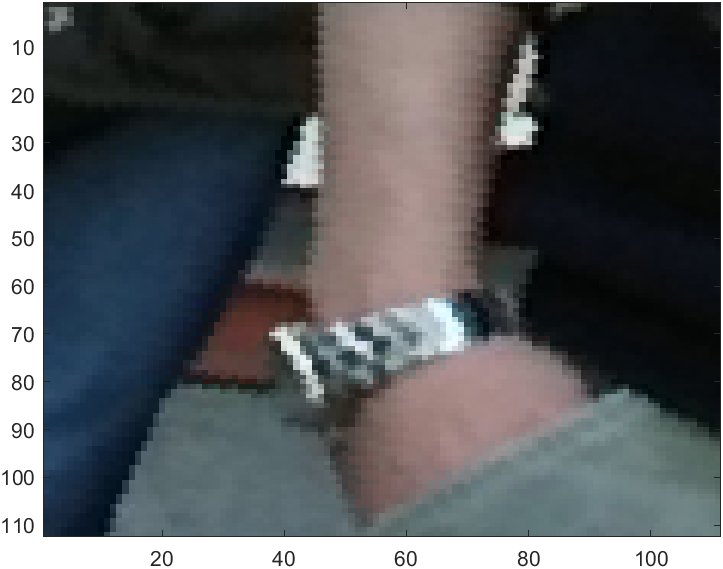
\includegraphics[width=4cm]{img/1345-1.png} }}%
\qquad
\subfloat[\centering immagine a colori dell'area relativa alla depth map con "cornice aggiuntiva"]{{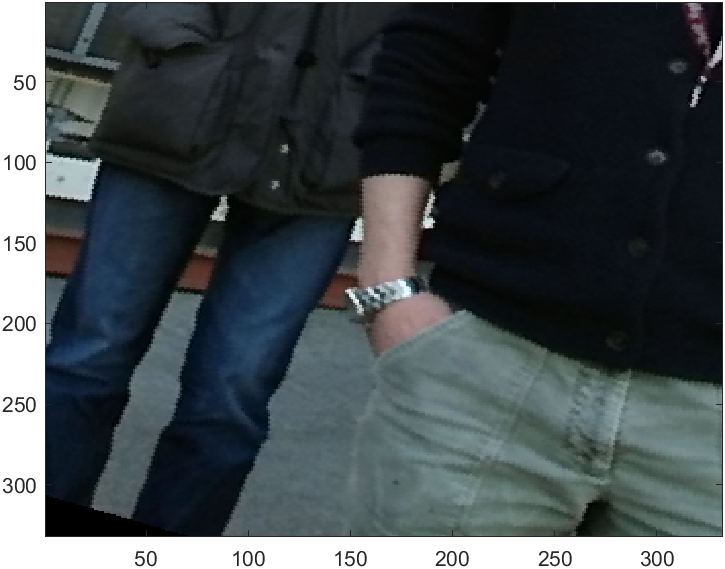
\includegraphics[width=4cm]{img/1345-2.png} }}%
\qquad
\subfloat[\centering Regressione parabolica sulla riga centrale una volta tolti i valori a 0]{{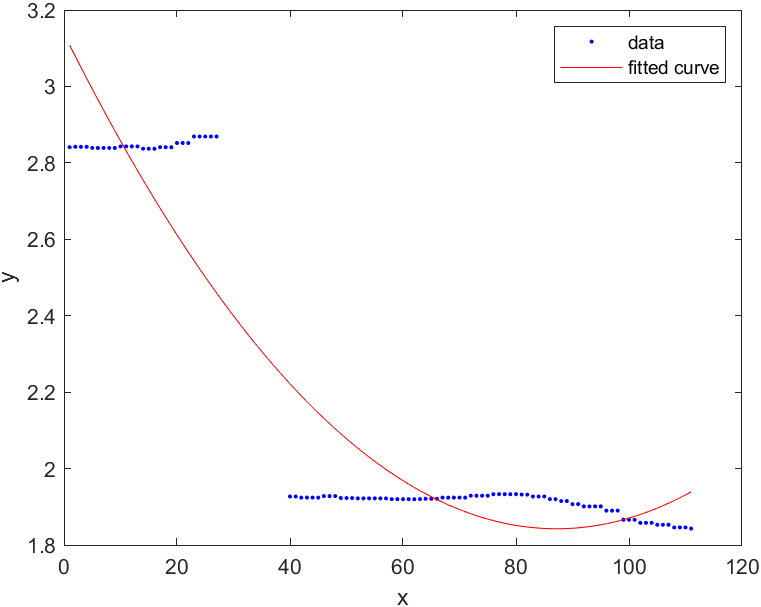
\includegraphics[width=4cm]{img/1345-3.png} }}%
\caption{Immagine 1345}
\end{figure}
La figura 6 mostra un caso in cui l'immagine a colori senza cornice aggiuntiva prende un'area con un oggetto chiaramente in primo piano, questo fa in modo che venga individuata come Face visto la sua regressione parabolica.

\hypertarget{legenda-file}{%
\section{Legenda file}\label{legenda-file}}

\begin{itemize}
\tightlist
\item
  metodo1.m contiene l'effettivo programma che controllando tutte le
  immagini presenti dentro DepthDATA salva nel vettore results se è
  faccia (0.5) o non faccia (1)
\item
  checkResults.m a partire dal vettore results, conteggia il numero di
  NonFace correttamente individuate o erratamente individuate
\item
  fixMatrix.m contiene la funziona fixMatrix che data una matrice di
  profondità sostituisce i valori 0 con il massimo della profondità
\item
  testValori.m testa i vari valori di marginRate (da 0.3 a 0.7)
  calcolandone di volta in volta Precision e Recall. Alla fine mostra
  l'andamento del tutto
\item
  risultatiTestValori.fig mostra il grafico risultante dall'esecuzione
  del file testValori.m con l'andamento di Precision e Recall.
\end{itemize}

\end{document}
